\documentclass[a4paper,12pt,UTF8]{ctexart}

% if you need to pass options to natbib, use, e.g.:
\PassOptionsToPackage{numbers, compress}{natbib}
% before loading nips_2016
%
% to avoid loading the natbib package, add option nonatbib:
% \usepackage[nonatbib]{nips_2016}

%\usepackage{nips_2016}

% to compile a camera-ready version, add the [final] option, e.g.:
\usepackage[final]{finalreport}

\usepackage[utf8]{inputenc} % allow utf-8 input
\usepackage[T1]{fontenc}    % use 8-bit T1 fonts
\usepackage{hyperref}       % hyperlinks
\usepackage{url}            % simple URL typesetting
\usepackage{booktabs}       % professional-quality tables
\usepackage{amsfonts}       % blackboard math symbols
\usepackage{nicefrac}       % compact symbols for 1/2, etc.
\usepackage{microtype}      % microtypography
\usepackage{CJKutf8}
\usepackage{graphicx}
\usepackage{float}
\usepackage{amsmath}
\usepackage{pdfpages}
\usepackage{titlesec}
\usepackage{indentfirst}

\setlength{\parindent}{2em}

\newcommand{\norm}[1]{\left\lVert#1\right\rVert}

\title{《人工神经网络》大作业最终报告:神经图像编辑}


% The \author macro works with any number of authors. There are two
% commands used to separate the names and addresses of multiple
% authors: \And and \AND.
%
% Using \And between authors leaves it to LaTeX to determine where to
% break the lines. Using \AND forces a line break at that point. So,
% if LaTeX puts 3 of 4 authors names on the first line, and the last
% on the second line, try using \AND instead of \And before the third
% author name.

\newcommand{\song}{\CJKfamily{zhsong}}	% 宋体
\newcommand{\hei}{\CJKfamily{zhhei}}	% 黑体
\newcommand{\fs}{\CJKfamily{zhfs}}		% 仿宋
\newcommand{\kai}{\CJKfamily{zhkai}}	% 楷体
\newcommand{\li}{\CJKfamily{zhli}}		% 隶书
\newcommand{\you}{\CJKfamily{zhyou}}	% 幼圆

\author{
  徐鉴劲 \\
  2015011313 \\
  计算机科学与技术系 \\
  清华大学 \\
  \texttt{xujj15@mails.tsinghua.edu.cn}
  %% examples of more authors
  \AND
  贾越凯 \\
  2015011335 \\
  计算机科学与技术系 \\
  清华大学 \\
  \texttt{jiayk15@mails.tsinghua.edu.cn} \\
  \AND
  寇明阳 \\
  2015011318 \\
  计算机科学与技术系 \\
  清华大学 \\
  \texttt{kmy15@mails.tsinghua.edu.cn} \\
  %% \And
  %% Coauthor \\
  %% Affiliation \\
  %% Address \\
  %% \texttt{email} \\
}

\begin{document}

\maketitle

\begin{abstract}

\end{abstract}


\section{引言}

图像是人类重要的交互途径,然而大部分人却不具有绘画的才能,本项目意图在于以人工智能的手段降低非专业人士在绘图方面的技术壁垒。在我们的作品神经图像编辑中,用户给出简笔画就可以得到算法生成的与预期相似的图画;用户还可以继续完善简笔画,对图像进行符合人类直觉的图像编辑,达到更符合预期的结果。
通过简笔画生成图像的技术有着广泛的应用前景,例如基于草图的商品搜索,适用于个体创作人的插图绘制,面向兴趣爱好者的辅助工具等等。

神经图像编辑的范围十分广阔,本项目研究动漫头像编辑这一子类上的应用。

经过一个学期的时间,我们的项目取得了如下成果:

\begin{enumerate}
\item 成功复现了高质量的动漫人物头像生成网络。
\item 成功应用编辑图像方法于极深层的神经网络。
\item 获得了高于基线的生成成果和编辑成果。包括生成真实度上升,生成清晰度上升($64 \times 64 \Rightarrow 128 \times 128$)和肉眼可见的编辑质量上升
\item 基于Web/Server的交互界面。
\end{enumerate}

\begin{figure}[H]
  \centering
  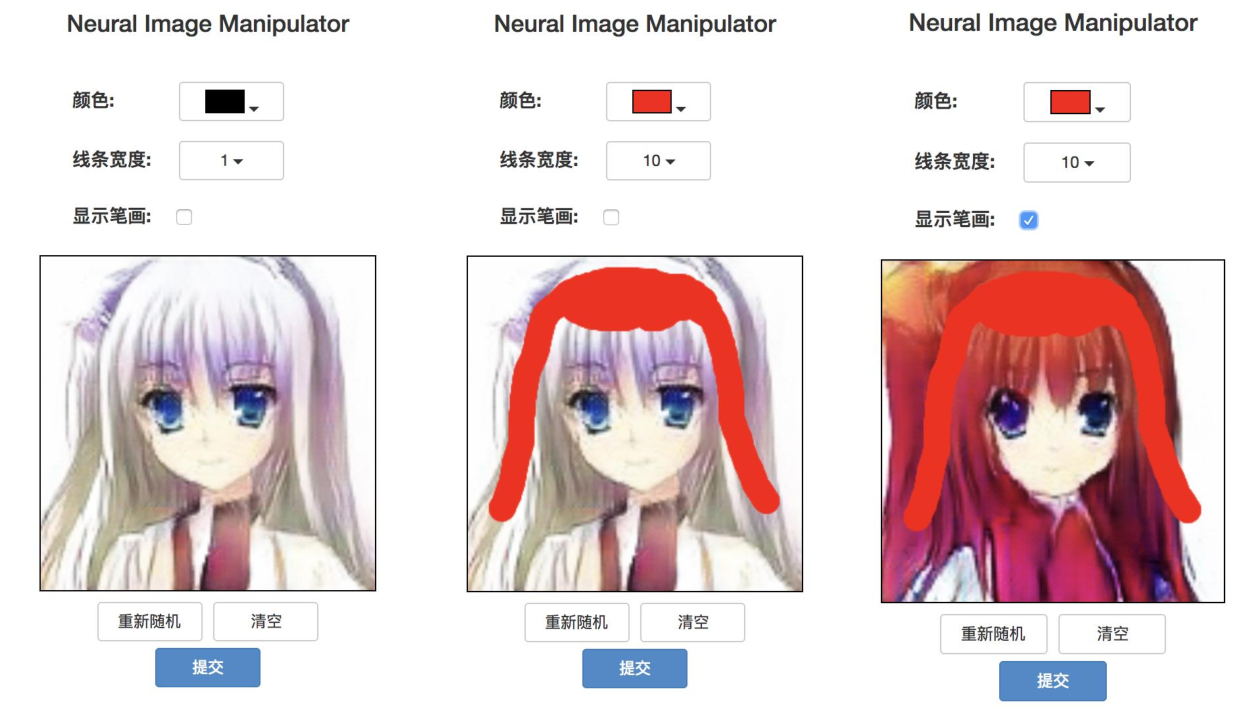
\includegraphics[width=0.9\linewidth]{figs/frontend.pdf}
  \caption{\kai 项目效果展示。用户通过网页前端绘制简笔画,提交到后台,经过神经网络的优化编辑以后,返回一个符合编辑预期的图像。}
  \label{fig:frontend}
\end{figure}


\section{相关工作}


现有的研究中,与草图生成图像相关的研究可以分为两类,一类是使用语义图像作为输入的条件生成网络,一类是将编辑过程看作可优化的过程,调整生成器的输入的方法。前一类以pix2pix为代表~\cite{isola2016image},输入一个精确的语义地图(semantic segmentation map),每一个像素表明了所属的物体类别,通过一个变化后的AutoEncoder输出生成图像。后一类使用普通的生成网络,接受随机向量的输入,输出生成图像,通过设计一种改变输入随机向量的方法来使得网络生成靠近期望结果的输出。

由于动漫人脸生成任务的约束,我们没有语义精确的数据集,难以按照原文复现第一类方法,所以不与之比较。本项目比较的baseline主要有两个,一个是交互式生成对抗网络iGAN~\cite{Zhu2016Generative},一个是神经图像编辑器Neural Photo Editor~\cite{Brock2016Neural}。这两个均可以完成编辑功能,然而他们的问题主要有:

\begin{enumerate}
\item 生成精度低。这两个工作并没有将编辑的操作应用在强大的生成网络上,生成的精度最高只能达到64x64。
\item 没有应用于动漫画风的领域上。这两个工作的数据集都是较为完善的真实数据集图片,如户外风景和人类图片数据集,然而本项目中涉及到的动漫数据集属于难度较高的类型,是从网络上爬取的数据集、规模较小、画风多样、混杂有低质量图片等等。
\item 编辑中有很大的可能丧失图片类别的特性,丧失人脸的特征。
\end{enumerate}

这些问题在下面的例子中都有体现,然而下面的例子已经是经过多次尝试而得到的最好结果。

\begin{figure}[H]
  \centering
  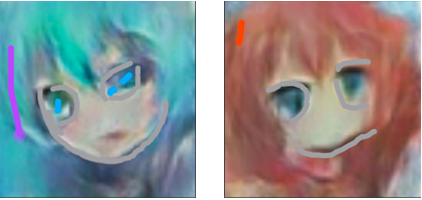
\includegraphics[width=0.9\linewidth]{figs/baseline1.PNG}
  \caption{\kai iGAN在收集到的Getchu数据集上的复现,使用iGAN开源的代码,遵循了原文的设置。图中灰色线条是边缘简笔画,其他的彩色线条是颜色简笔画,图片是在这些简笔画限制下的编辑结果。在生成的过程中经理了频繁的失败,极易丧失生成结果的真实行。展示的图片经过了精心挑选,达到了iGAN所能达到的最佳效果,然而结果仍然十分不美观。}
  \label{fig:baseline1}
\end{figure}

\begin{figure}[H]
  \centering
  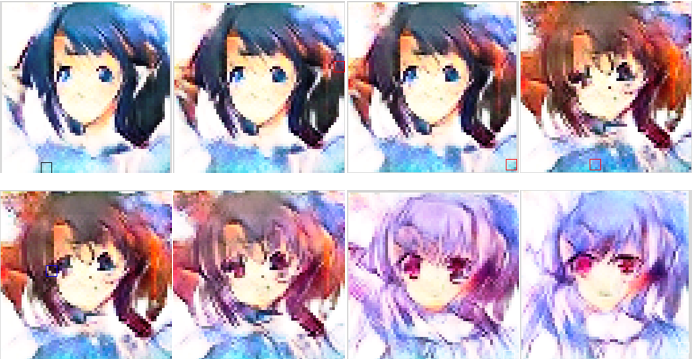
\includegraphics[width=0.9\linewidth]{figs/baseline2.PNG}
  \caption{\kai Neural Photo Editor (NPE) 在Getchu数据集上的复现,使用了NPE开源的代码,遵循了原文的设置。从左上到右下是在神经图像编辑过程中顺序产生的,用户在1~5张中头发的位置画了红色线条,并在 6~8张中画了蓝色线条。头像颜色变化基本与预期相符,体现了编辑的有效性。}
  \label{fig:baseline2}
\end{figure}

\section{方法}

\subsection{框架}

我们的项目分为两个阶段实现,第一阶段不编辑一个给定的具体图像,先考虑编辑一个随机生成的图像,如图 \ref{fig:workflow1};第二阶段再加入一个编码网络来完成对于具体图像的编辑,在图 \ref{fig:workflow2} 中进行了说明。目前我们已经完成了第一个阶段的工作,第二个阶段完成了网络的训练,正在进行前端的调整,以支持上传图像并编辑的功能。

\begin{figure}[H]
  \centering
  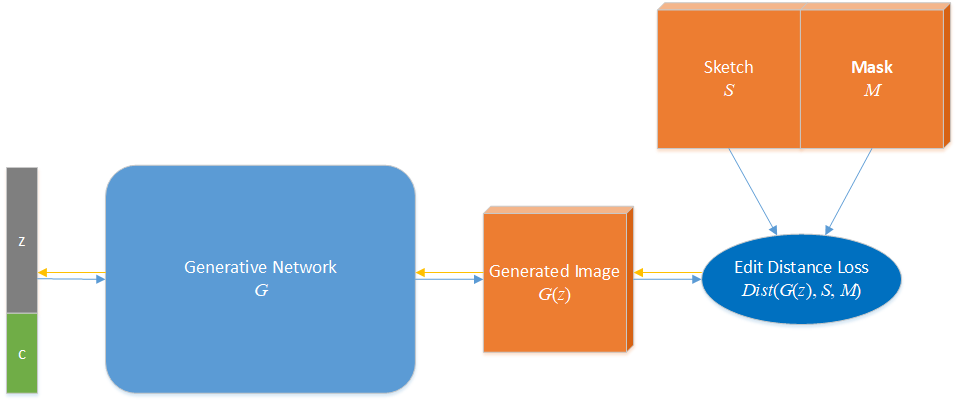
\includegraphics[width=1\linewidth]{figs/workflow1.png}
  \caption{\kai 第一阶段的项目解决方法。从随机向量出发,由生成网络生成初始结果,用户给定简笔画和对应的遮罩,由编辑距离函数计算误差和倒数,并借此更新 $z$,达到编辑图像的目的。蓝箭头表示数据流向,橙色箭头表示导数。}
  \label{fig:workflow1}
\end{figure}

\begin{figure}[H]
  \centering
  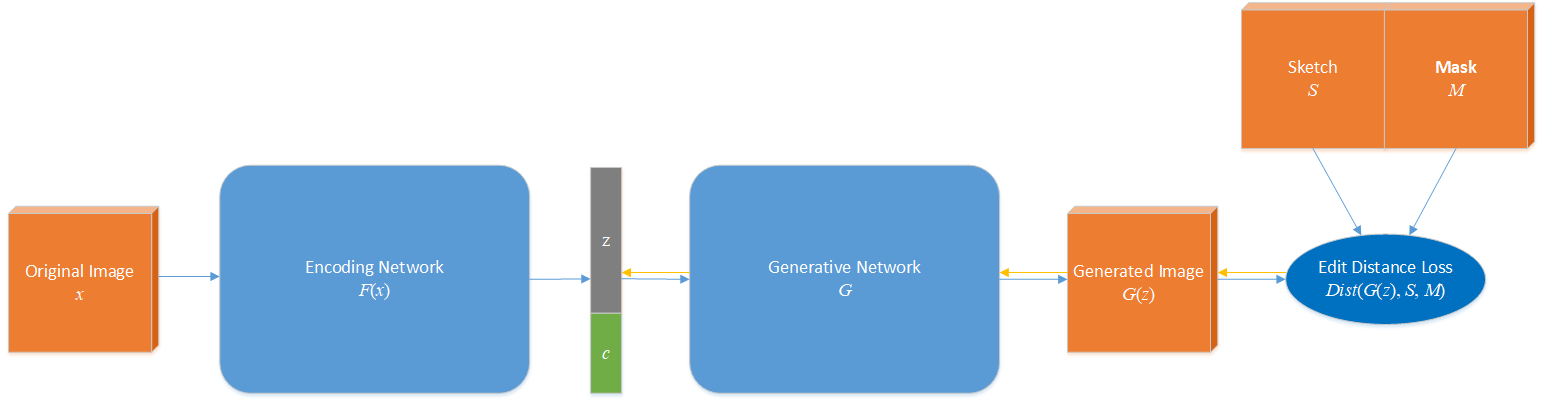
\includegraphics[width=1\linewidth]{figs/workflow2.png}
  \caption{\kai 第二阶段的项目解决方法。从一个待编辑图像出发,先通过编码网络生成 $z$ 与 $c$,然后经过生成网络生成重构结果,用户给定简笔画和对应的遮罩,由编辑距离函数计算误差和导数,并借此更新 $z$,达到编辑图像的目的。蓝箭头表示数据流向,橙色箭头表示导数。}
  \label{fig:workflow2}
\end{figure}

\subsection{编辑图像}

一个生成网络$G(z, c)$接受随机向量$z$(遵循高斯分布)和条件向量$c$作为输入,生成图像$I = G(z, c)$。同时用户给定编辑图像$I'$,例如一副简笔画,则可以据此给出生成图像与编辑图像之间的距离$Dist(G(z, c), I')$。设$I$在像素点$(i, j)$处的RGB颜色向量为$I_{ij}$。定义$M_{ij}$为像素点$(i, j)$处的Mask向量,含义是用户编辑的部分是否包含像素点$(i, j)$。$M_{ij}$的值只可能为全$0$或全$1$,定义如下:

\begin{equation}
  M_{ij} =
  \begin{cases}
    [0, 0, 0]   &  \text{if $\norm{I'_{ij}} = 0$} \\
    [1, 1, 1]   &  \text{if $\norm{I'_{ij}} \neq 0$}
  \end{cases}
\end{equation}

则我们可以基于已有的$M_{ij}$、$I_{ij}$和$I'_{ij}$定义原生成图像与编辑图像之间的距离,这里的距离定义为两幅图中每个用户编辑的像素点距离的$L1 norm$除以一个合理的代表用户修改总点数的值。这样定义的目的是为了仅仅对用户编辑的位置进行修改,且提供与修改像素点数无关的距离函数,避免用户修改的点过少时效果变差。即定义

\begin{equation}
  Dist(I, I') = \frac{\sum_{ij} |I_{ij} - I'_{ij}| \cdot M_{ij}}{1 + \sum_{ij} M_{ij}}
\end{equation}

假设 $G$ 已经得到,本文的基本目标是求使$Dist(G(z, c), I')$最小的$z$和$c$:

\begin{equation}
  \arg\min_{z, c} Dist(G(z, c), I')
\end{equation}

设学习率为$lr$。为求这样的$z$和$c$,先给出随机的合法初值$z_{0}$和$c_{0}$,再将距离函数对$z_{0}$和$c_{0}$求偏导:

\begin{equation}
  \Delta z_{0} = \frac{\partial}{\partial z} Dist(G(z_{0}, c_{0}), I')
\end{equation}
\begin{equation}
  \Delta c_{0} = \frac{\partial}{\partial c} Dist(G(z_{0}, c_{0}), I')
\end{equation}

之后,在$z$和$c$的反函数域上以学习率$lr$使用Gradient Descent算法进行学习,并限制$\tilde z_{1}$和$\tilde c_{1}$在合法的边界中:
\begin{equation}
  \tilde z_{1} = arc \tanh z_{0} - lr \cdot \Delta z_{0}
\end{equation}

\begin{equation}
  \tilde c_{1} = - \log (\frac{1}{c_{0}} - 1) - lr \cdot \Delta c_{0}
\end{equation}

最后,将$\tilde z_{1}$和$\tilde c_{1}$变换回原来的函数域,得到新的值$z_{1}$和$c_{1}$:

\begin{equation}
  z_{1} = \tanh (\tilde z_{1})
\end{equation}
\begin{equation}
  c_{1} = [ sigmoid(\tilde c_{1}) ]
\end{equation}

重复这样的学习,即可使$Dist(G(z, c), I')$不断减小,直到生成符合要求的图片。

% --- 审核:要求能看懂 -- 【jyk】

\subsection{训练网络}

本项目中对于多种网络结构和训练方法进行了尝试,最终确定了和~\cite{Jin2017Towards}类似的网络结构与训练方法。我们采用了使用多层Residual Block ~\cite{he2016deep} 搭建的深层生成器和判别器,使用DRAGAN ~\cite{kodali2017convergence}加上辅助分类器~\cite{odena2016conditional}的训练方法进行。

设真实数据集为$D_R$,一个训练样例可以表示成$x \sim P_r$,同时随机向量 $z$ 和 $c$ 有$z \sim P_z$和$c \sim P_c$。构造一个判别网络$D(I)$。

\begin{equation}
  \min_{\theta_G,\theta_f} \max_{\theta_D} \mathbb{E}_{(x, z, c) \sim (P_r, P_z, P_c)} \Big[ \log D(x) + \log\big(1 - D(G(z, c))\big) + \log\big(1 - D(G(f(x)))\big)\Big]
\end{equation}

进一步地,使用DRAGAN的训练可以用如下公式表达

\begin{equation}
\begin{aligned}
  \mathcal{L}_{adv}(D) &= -\mathbb{E}_{x\sim P_{data}}[\log D(x)] - \mathbb{E}_{x\sim P_{noise},c\sim P_{cond}}\big[\log(1-D(G(z,c)))\big] \\
  \mathcal{L}_{cls}(D) &= \mathbb{E}_{x\sim P_{data}}\big[\log P_D[label_x|x]\big] + \mathbb{E}_{x\sim P_{noise},c\sim P_{cond}}\Big[\log\big(P_D[c|G(z,c)]\big)\Big] \\
  \mathcal{L}_{gp}(D) &= \mathbb{E}_{\tilde{x}\sim P_{perturebed\_data}}\left[\big(\norm{\nabla_{\tilde{x}}D(\tilde{x})}_2-1\big)^2\right] \\
  \mathcal{L}_{adv}(G) &= \mathbb{E}_{x\sim P_{noise},c\sim P_{cond}}\big[\log D(G(z,c))\big] \\
  \mathcal{L}_{cls}(G) &= \mathbb{E}_{x\sim P_{noise},c\sim P_{cond}}\big[\log P_D[c|G(z,c)]\big] \\
  \mathcal{L}(D) &= \mathcal{L}_{cls}(D) + \lambda_{adv}\mathcal{L}_{adv}(D) + \lambda_{gp}\mathcal{L}_{gp}(D) + \lambda_{reg} \mathcal{L}_{2}(D) \\
  \mathcal{L}(G) &= \lambda_{adv}\mathcal{L}_{adv}(G) + \mathcal{L}_{cls}(G) + \lambda_{reg} \mathcal{L}_{2}(D)
\end{aligned}
\end{equation}

其中$\tilde{x}$是经过扰动的真实数据,

\begin{equation}
\tilde{x} = x + 0.5 \times \alpha std(x) \\
\alpha ~ uniform(0, 1)
\end{equation}

\section{实验}

\subsection{生成对抗训练}

在我们完成项目的过程中,在MNIST数据集和自定义的Getchu数据集上都进行了多次实验,包括网络结果的选取,普通GAN训练,WGAN~\cite{2017arXiv170107875A}和DRAGAN训练方法。

% -- MNIST --

% -- 训练设置 -- 【徐鉴劲】

% -- IAN与DRAGAN的对比 -- 【徐鉴劲】

% -- GETCHU -- 【徐鉴劲】

% -- DRAGAN网络的loss图、中间演变 -- 【徐鉴劲】

\subsection{图像编辑}

% -- 实际设置 -- 【寇明扬】
%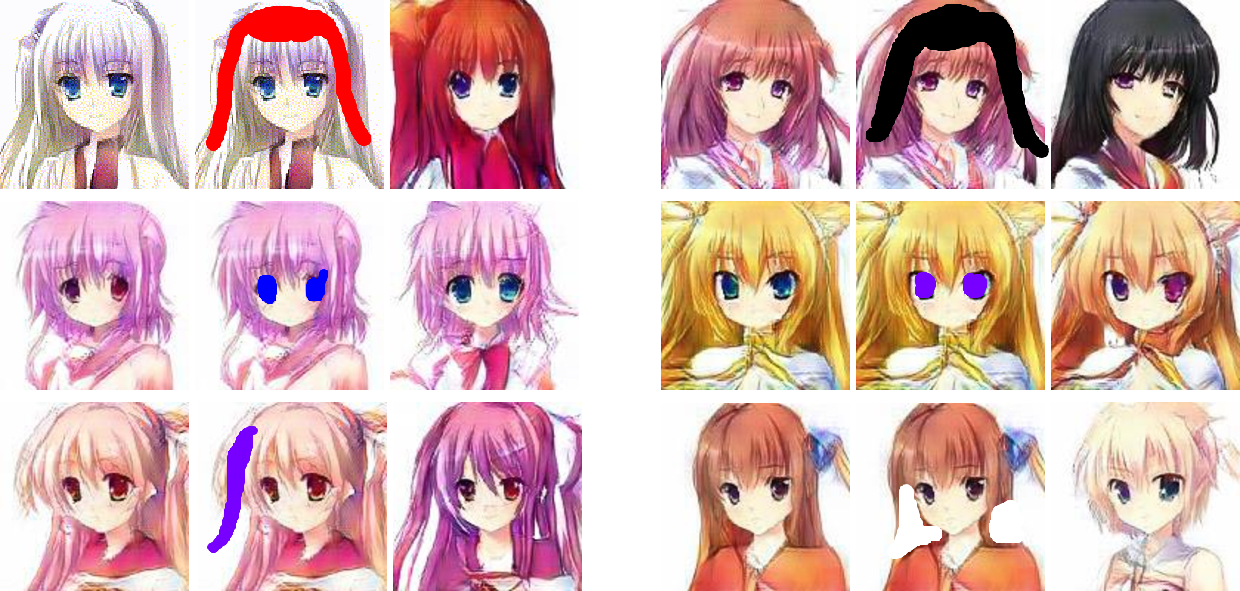
\includepdf[addtotoc={1,section,1,title in toc,cc},pages=1,offset=0cm 0.5cm]{figs/pic.pdf}

下面展示几组图像编辑效果的样例,如图3和图4所示。

\begin{figure}[H]
  \centering
  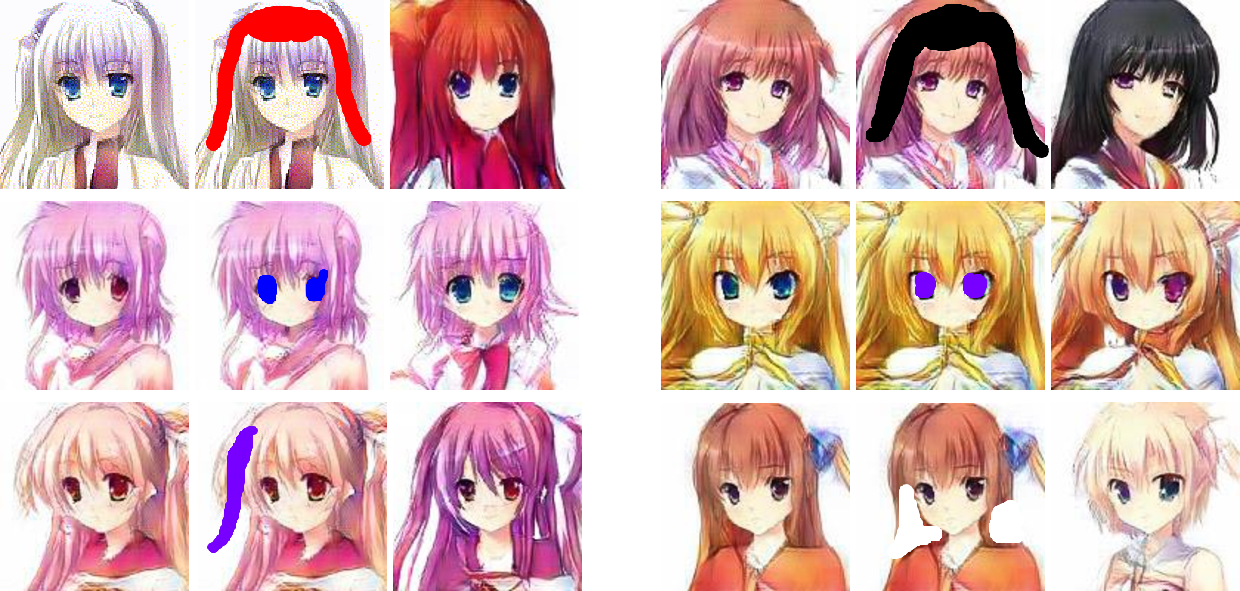
\includegraphics[width=0.9\linewidth]{figs/pic.pdf}
  \caption{\kai 编辑效果展示,共六组,每组三幅图。每组中最左边的一幅为原图,中间的一幅图为编辑图,最右边的一幅图为生成的结果图。第一行的两组为更换发色的例子,可以看出,左边的一组成功将原图中的人物的发色从白色变成了红色,而右边的一组成功将原图中的人物的发色从红色变成了黑色。第二行的两组为更换瞳色的例子,左边的一组成功将人物瞳色从红色变成了蓝色,而右边的一组将人物瞳色从蓝色变成了紫红色。第三行的两组为更换发型的例子,左边的一组成功在人物头上添加了一束紫色的头发,而右边的一组成功去掉了人物头两侧的头发,将人物从长发变成了短发。
  可以看出,我们生成的模型可以进行对动漫人物的发色、瞳色、发型等多方面特征进行编辑,且效果出色。}
  \label{fig:pic}
\end{figure}


% -- 选几张展示编辑效果(参考ppt) -- 【寇明扬】

% -- 结论 -- 【寇明扬】

\subsection{网页应用}

我们基于训练好的模型,构建了一个基于 B/S 架构的网页应用,可以通过 Web 浏览器进行在线图像编辑。

\subsubsection{网页端}
我们的网页端界面如图 \ref{figure:web1} $\sim$ 图 \ref{figure:web3}  所示,能够运行在任何一款现代浏览器上。

\begin{figure}[H]
  \begin{minipage}[t]{0.33\linewidth}
      \centering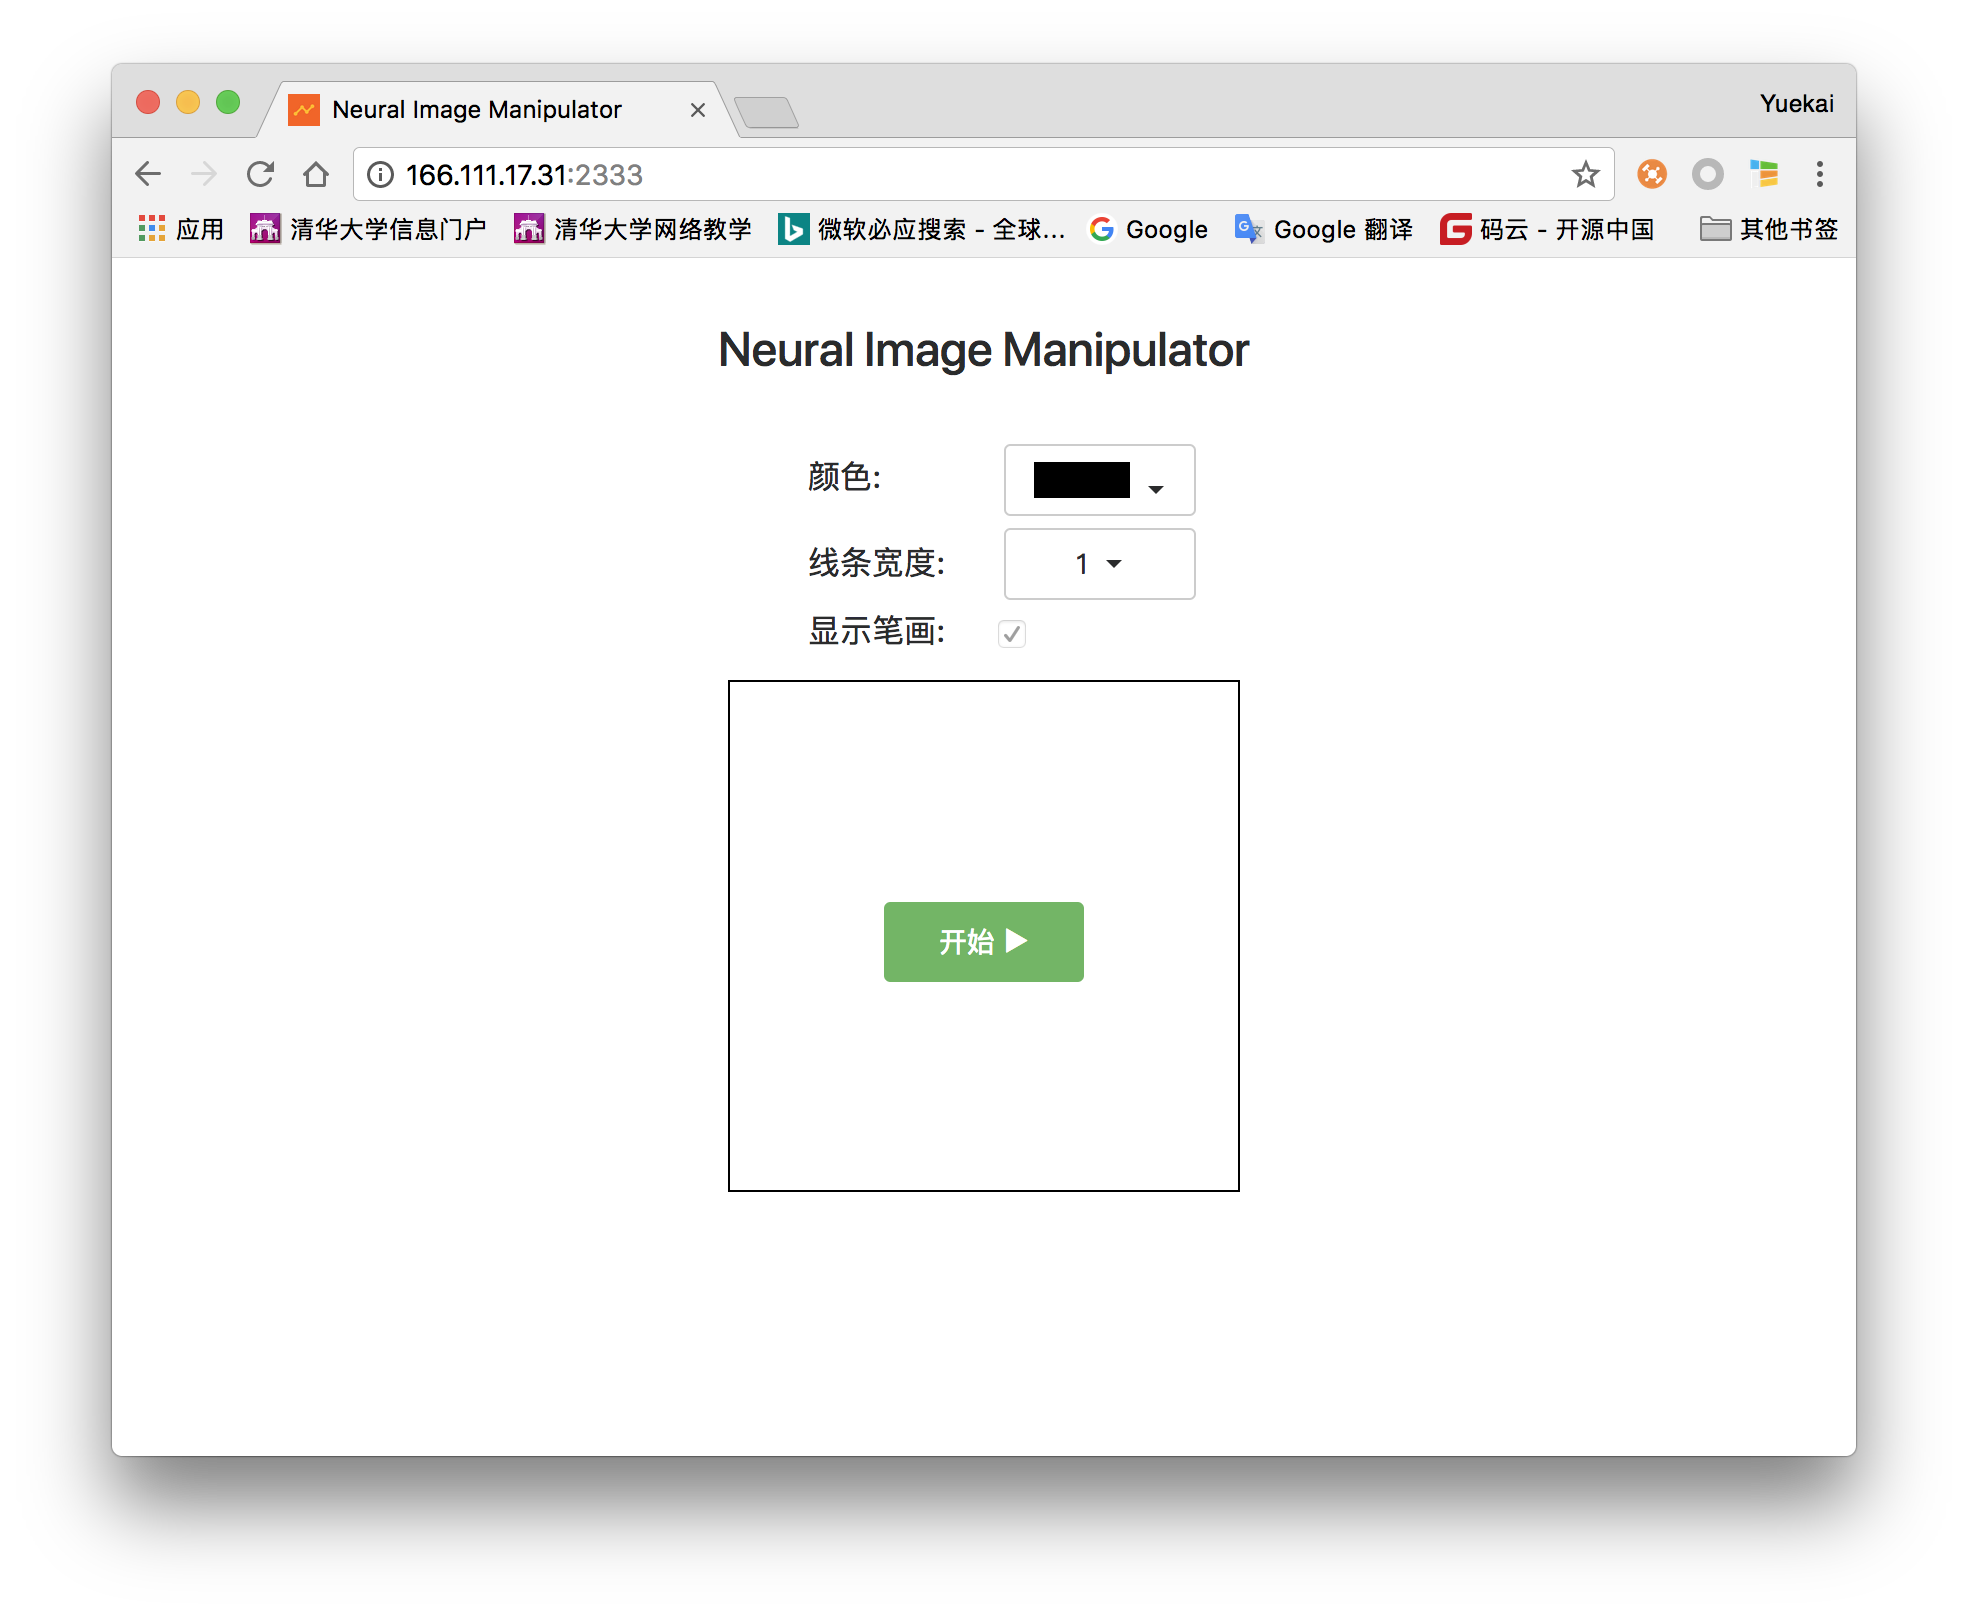
\includegraphics[height=4cm]{figs/web1.png}
      \caption{\kai 开始页面}\label{figure:web1}
  \end{minipage}%
  \begin{minipage}[t]{0.33\linewidth}
      \centering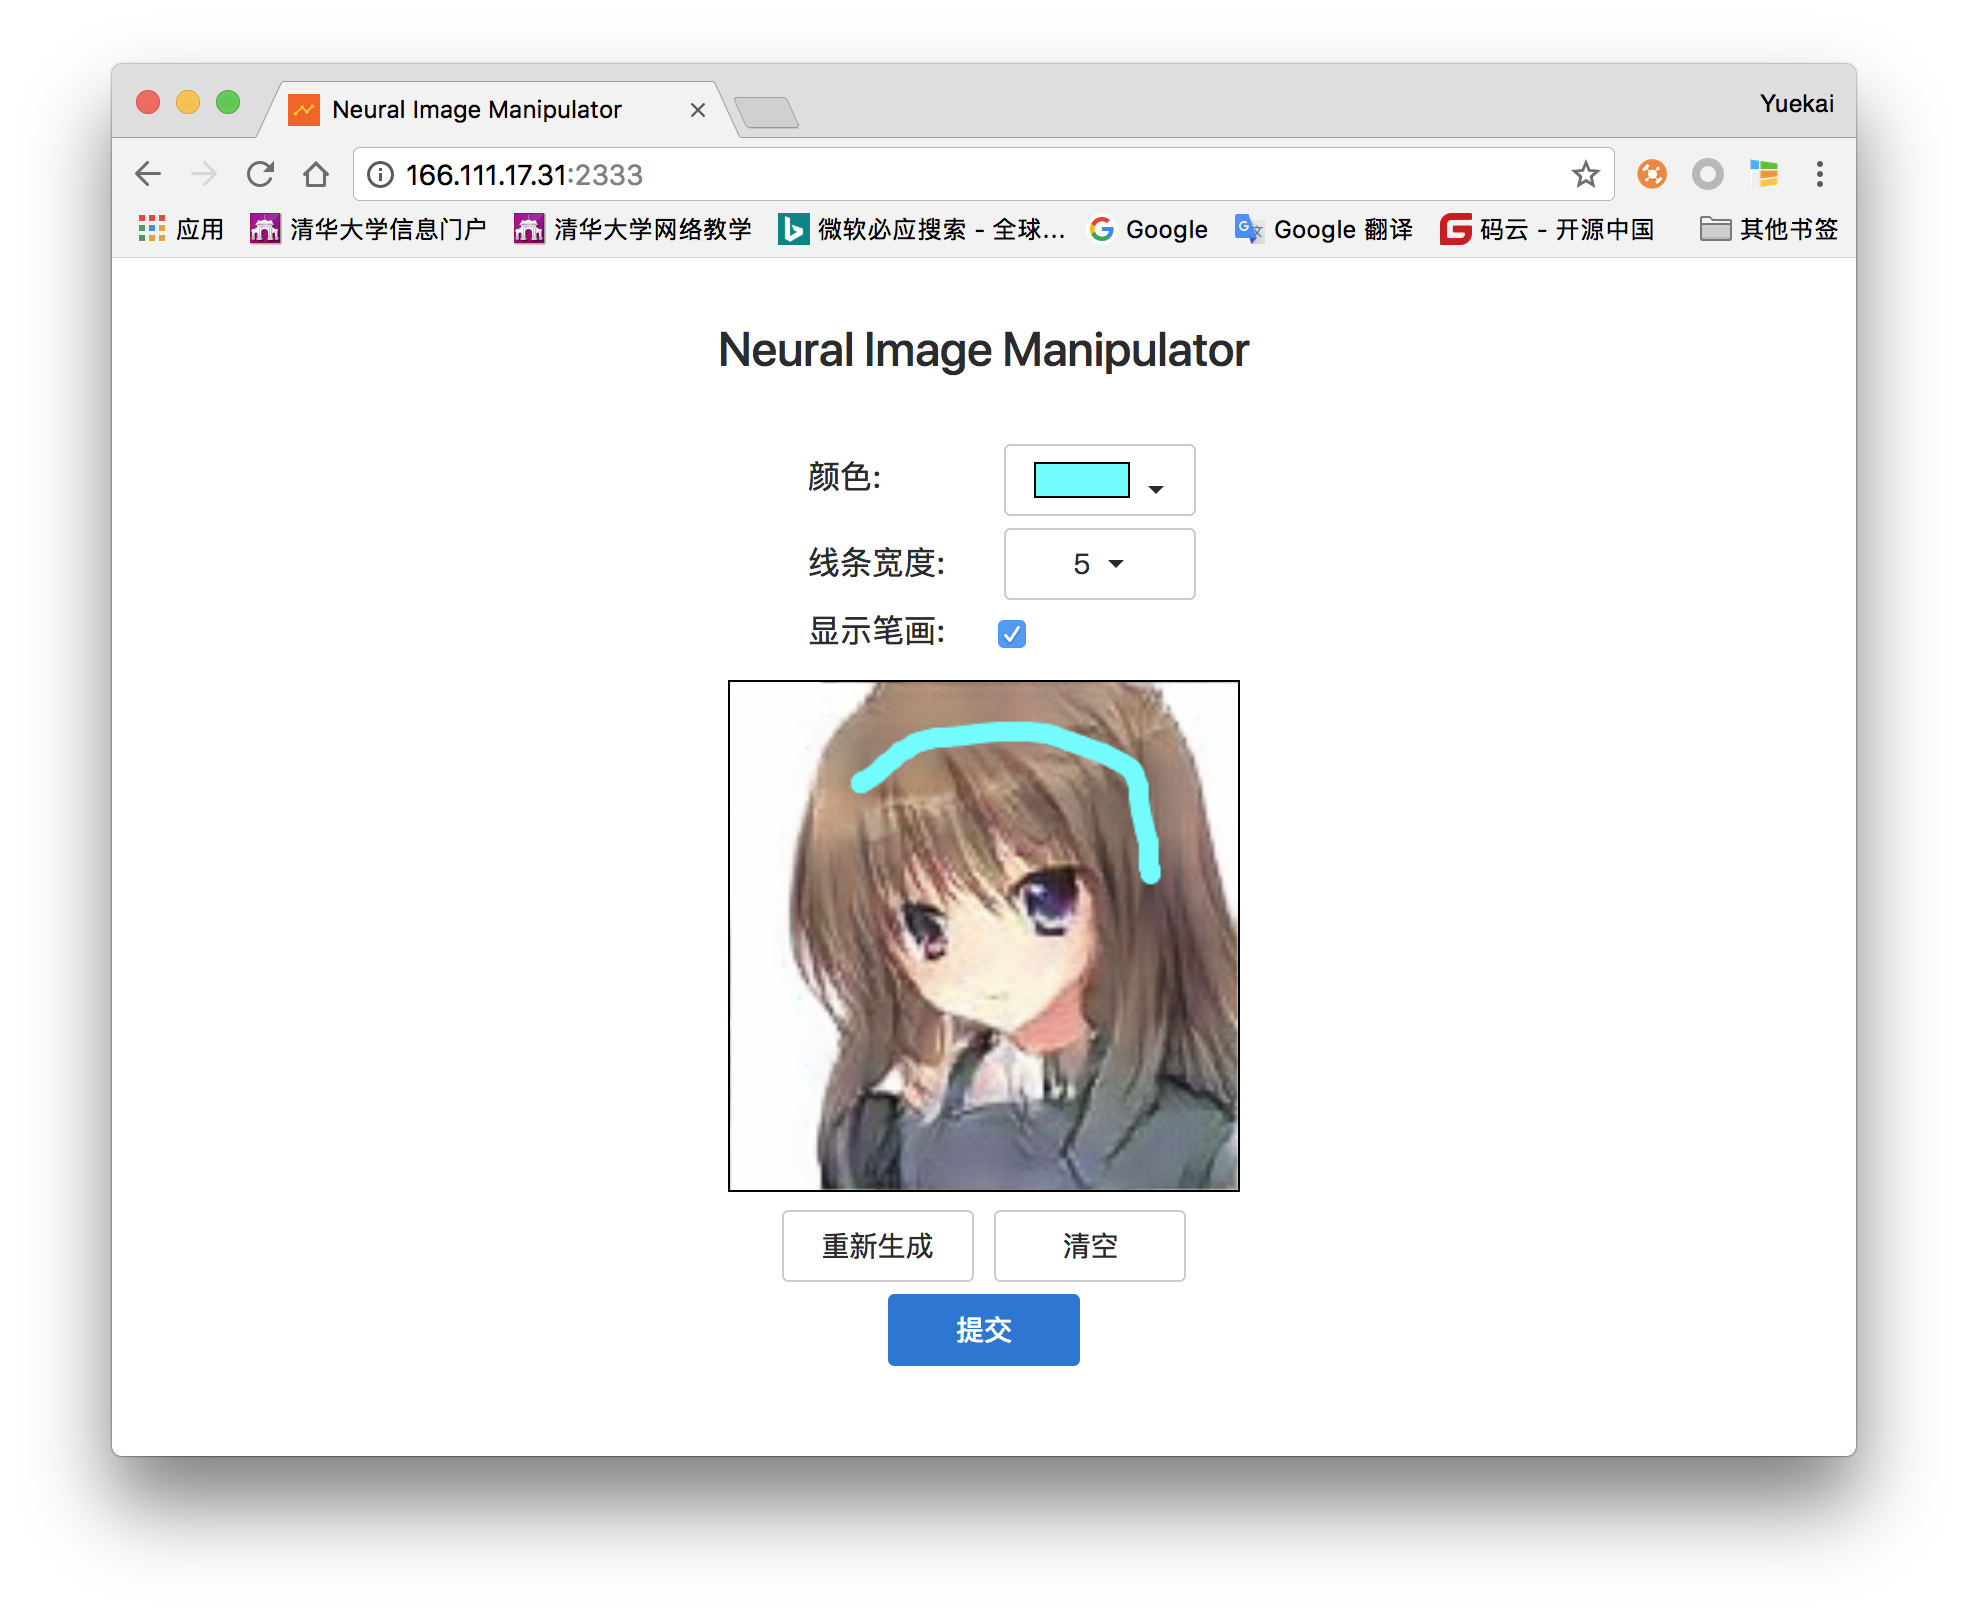
\includegraphics[height=4cm]{figs/web2.png}
      \caption{\kai 输入笔画}\label{figure:web2}
  \end{minipage}%
  \begin{minipage}[t]{0.33\linewidth}
      \centering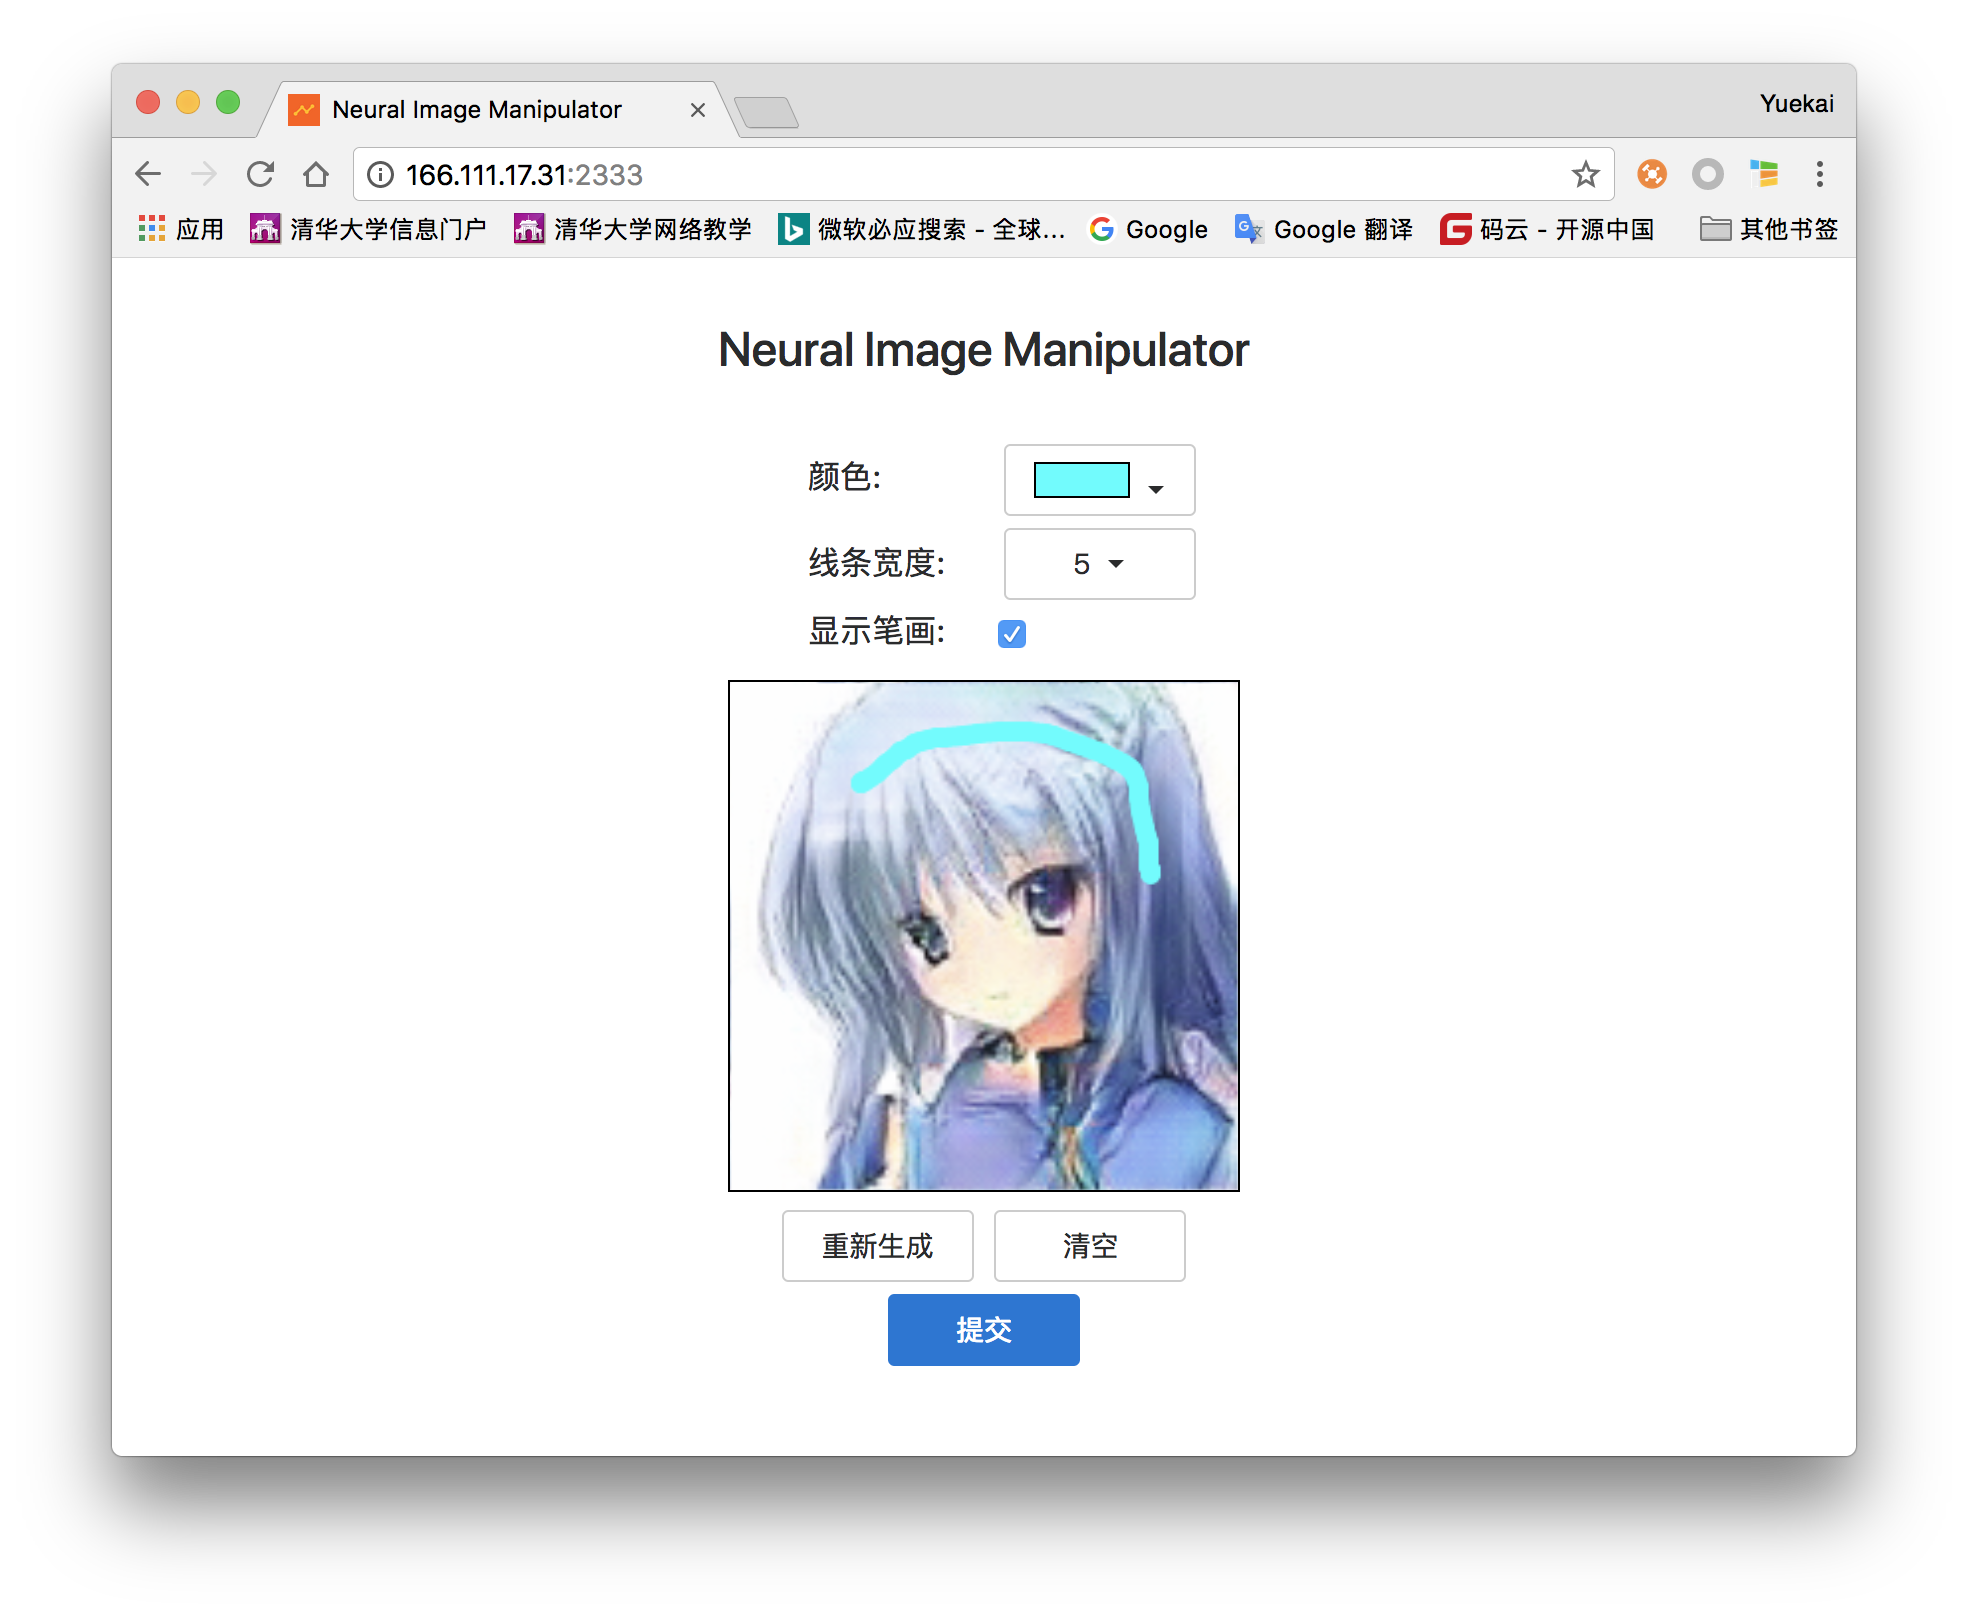
\includegraphics[height=4cm]{figs/web3.png}
      \caption{\kai 点击提交后}\label{figure:web3}
  \end{minipage}
\end{figure}

首次打开网页,点击 “开始按钮”,服务器会返回一张初始生成的图像。之后用户可以使用画笔工具,简单地勾勒出图片期望的变化方向,点击“提交”后,服务器就会返回在原图基础上,加上用户编辑条件后生成的图像;点击“重新生成”后,服务器会重新生成一张图片;点击“清空”能清空用户画的所有的笔画。此外,网页还支持更改画笔颜色、粗细,并能切换笔画的显示,以方便用户编辑。

该网页主要用 HTML 和 JavaScript 实现,并使用了 jQurey\footnote{\url{http://jquery.com}} 和 Bootstrap \footnote{\url{http://getbootstrap.com}} 等库。图片编辑框使用了 HTML5 的 \texttt{<canvas>},点击提交后,会将编辑框中的笔画图转成 Base64\footnote{\url{https://en.wikipedia.org/wiki/Base64}} 编码,使用 HTTP 请求发给服务器,之后服务器会返回生成图像的 Base64 编码,前端再将其作为图片编辑框的背景,显示给用户。

需要注意的是,用户每次点提交时,服务器是在该用户当前图像的基础上,再根据用户提供的笔画生成新图像,而且需要支持多用户同时编辑,即需要知道该用户当前的编辑状态。我们的做法是,服务器生成图像给前端时,会附带此时的 $z$ 和 $c$ 向量。前端将其保存下来,下次点提交时再发给服务器,服务器就会根据前端提供的 $z$ 和 $c$ 生成图像,以达到保存用户编辑状态的效果。

\subsubsection{服务器端}
由于训练模型使用的是 Python,所以我们选择了基于 Python 的 Django 框架搭建服务器端。

服务器端接收前端发来的笔画图,计算出 $sketch$ 和 $mask$ 矩阵,再根据前端发来的 $z$ 和 $c$,放入之前训练好的网络中,就能得到生成的图像。然后将其和修改后的 $z$ 和 $c$ 返回给前端。

实际测试时,模型的运行效率非常快,生成一张图像的时间约为 10 几毫秒,主要延时在于网络传输。因此,就算是多个用户同时访问网页进行编辑,服务器也完全可以承受住这样的负载。

\section{结论}

% -- 总结 -- 【徐鉴劲】

% -- 个人收获 ---【寇明扬】 【贾越凯】

\section*{参考文献}

\medskip

{\small
\bibliographystyle{ieee}
\bibliography{egbib}
}

\end{document}
